\section{User Interface}
The user interface of both the desktop and mobile client will be designed so that a user without a lot of technical knowledge of machine learning can easily make use of this web-tool. The user interface is also great for experienced engineers as it presents a simple and fast way to create models and start classifying data right away.

\subsection{Desktop}
The users are first met with a simple \hyperref[fig:login]{login/registration panel}. Then the \hyperref[fig:workspaces-list]{current workspaces} are listed, from which the users can choose to work with. The users can also \hyperref[fig:create-workspace]{create a new workspace}, in which they name it and choose the labels it will have. In the \hyperref[fig:workspace-overview]{workspace overview} page, the collected data samples are listed on the left, and on the right there are buttons to view the labels and models. The users can also easily select hyperparameters and train and deploy a model in this page with a single click.\hyperref[fig:workspace-link]{A link and a QR code}, which a mobile web client can use to start collecting data to this workspace, will also be available with a single click. Users can also see the \hyperref[fig:sample-overview]{data sample overview}, \hyperref[fig:labels-overview]{labels overview} and the \hyperref[fig:models-overview]{models overview}. Each model will provide \hyperref[fig:model-link]{its own link and QR code}, which a mobile client can use to start classifying actions with this mode and which again will be provided with a single click.

\subsection{Mobile}
When a QR Code is scanned or a link is visited, the users are met with a list of labels to choose from. When a label is selected, users are allowed to configure the recording parameters before pressing the button to start recording. After that, the countdown runs and then the recording page is displayed. In the end, it is stated that the recording is done. The users can repeat the recording process by pressing a redo button in this page or discard the previous recording.

Details of the mobile web client can be seen in the \hyperref[fig:mobile]{screenshots}.

\newpage

\subsection{Screenshots}

\begin{figure}[ht]
    \centering
    \fbox{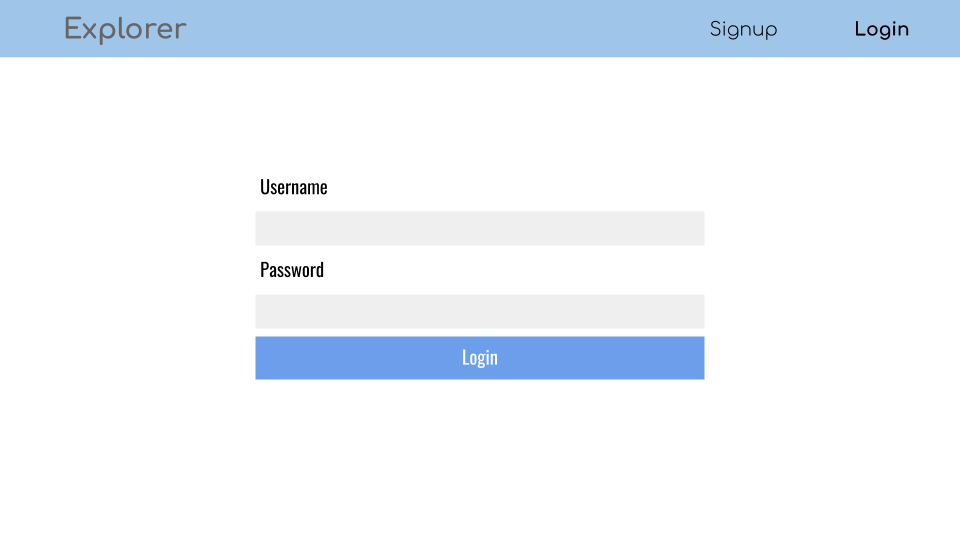
\includegraphics[width = .98\textwidth]{mockups/1.png}}
    \caption{Login/Registration Panel}
    \label{fig:login}
\end{figure}

\begin{figure}[!ht]
    \centering
    \fbox{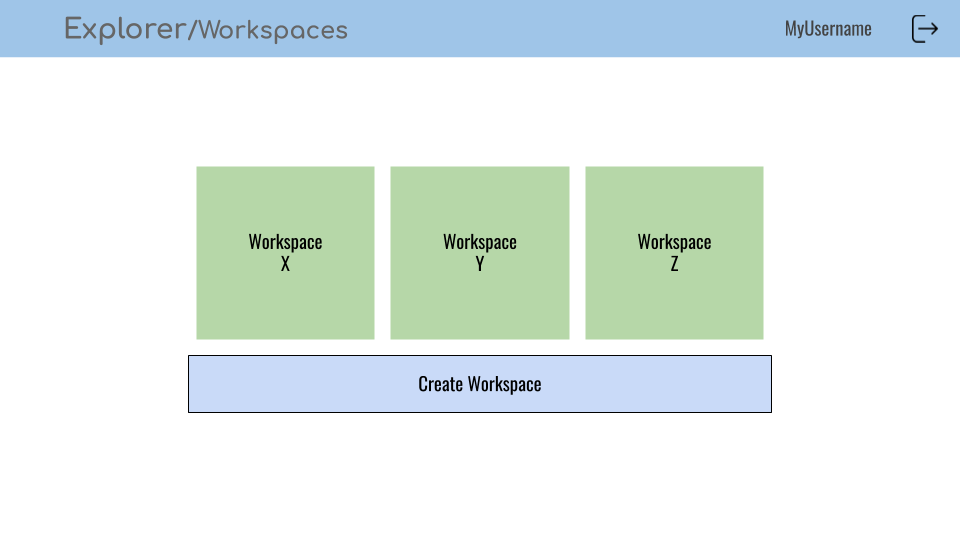
\includegraphics[width = .98\textwidth]{mockups/2.png}}
    \caption{List of current workspaces}
    \label{fig:workspaces-list}
\end{figure}

\begin{figure}[ht]
    \centering
    \fbox{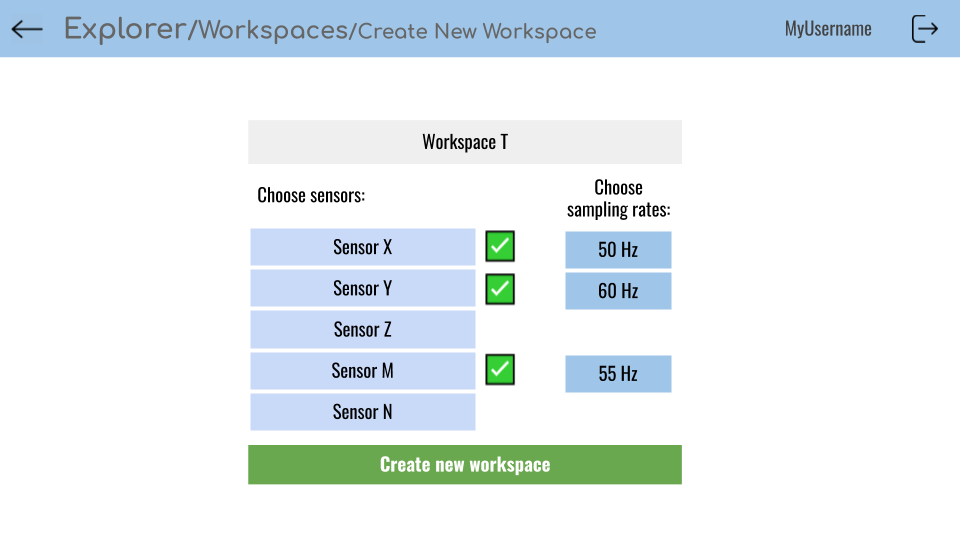
\includegraphics[width = .98\textwidth]{mockups/3.png}}
    \caption{Create a new workspace}
    \label{fig:create-workspace}
\end{figure}

\begin{figure}[ht]
    \centering
    \fbox{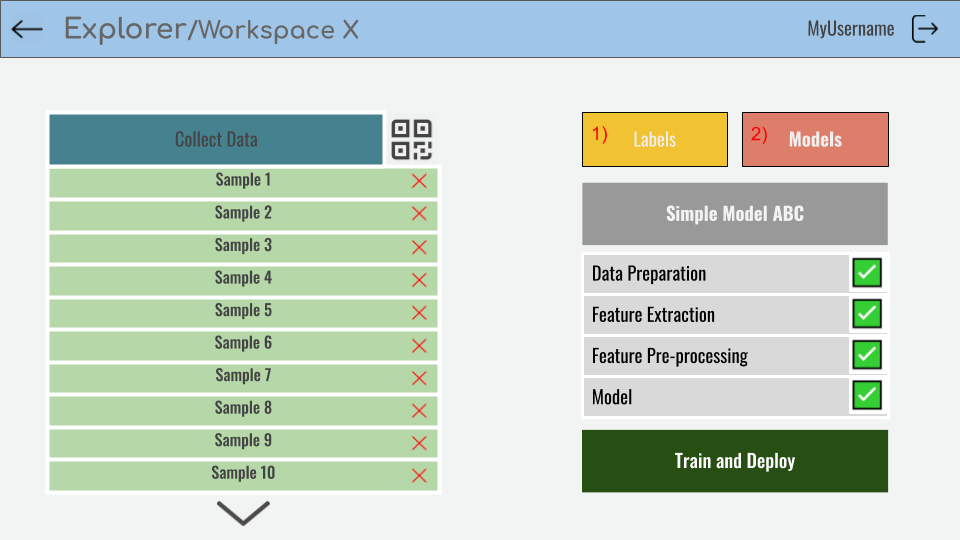
\includegraphics[width = .98\textwidth]{mockups/4.png}}
    \caption{Workspace overview}
    \label{fig:workspace-overview}
\end{figure}

\begin{figure}[ht]
    \centering
    \fbox{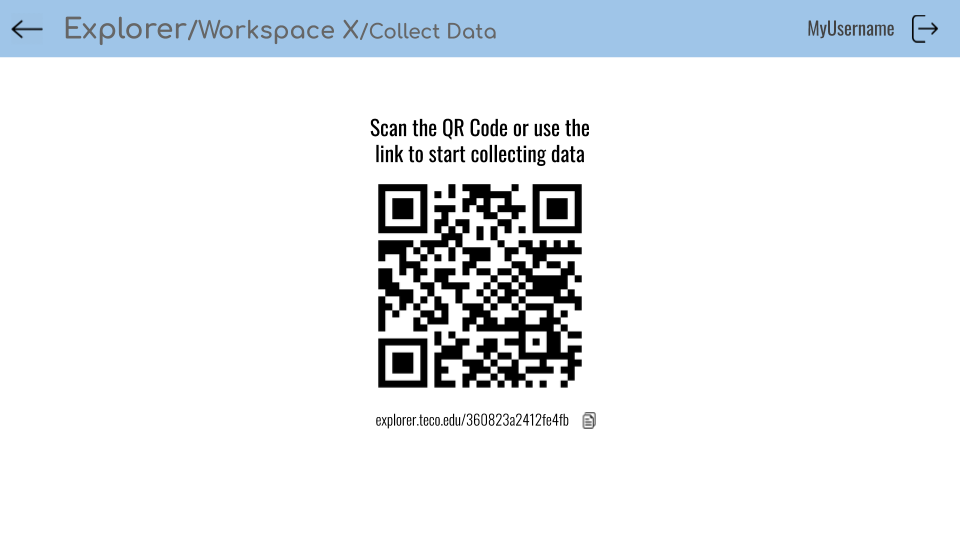
\includegraphics[width = .98\textwidth]{mockups/6.png}}
    \caption{QR Code/Link of workspace to collect data}
    \label{fig:workspace-link}
\end{figure}

\begin{figure}[ht]
    \centering
    \fbox{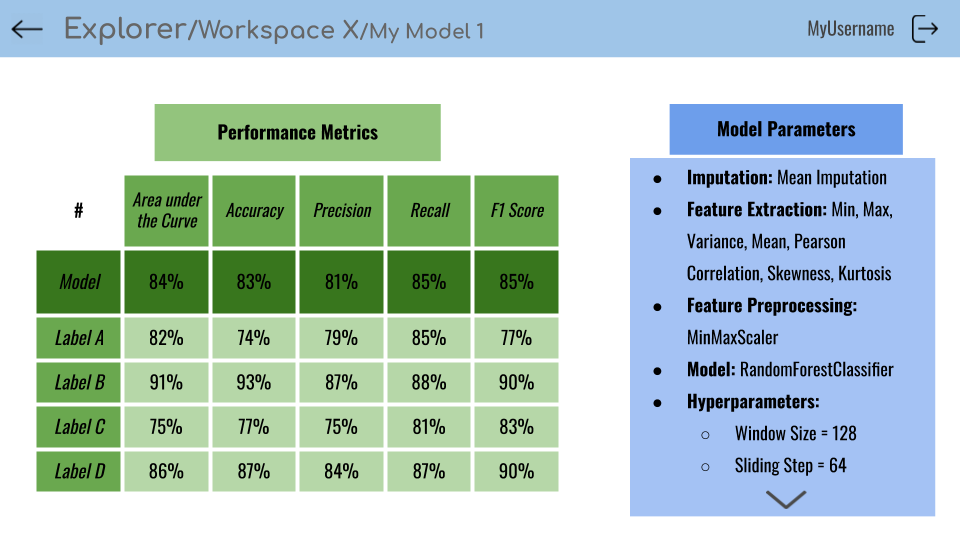
\includegraphics[width = .98\textwidth]{mockups/10.png}}
    \caption{Data sample overview}
    \label{fig:sample-overview}
\end{figure}

\begin{figure}[ht]
    \centering
    \fbox{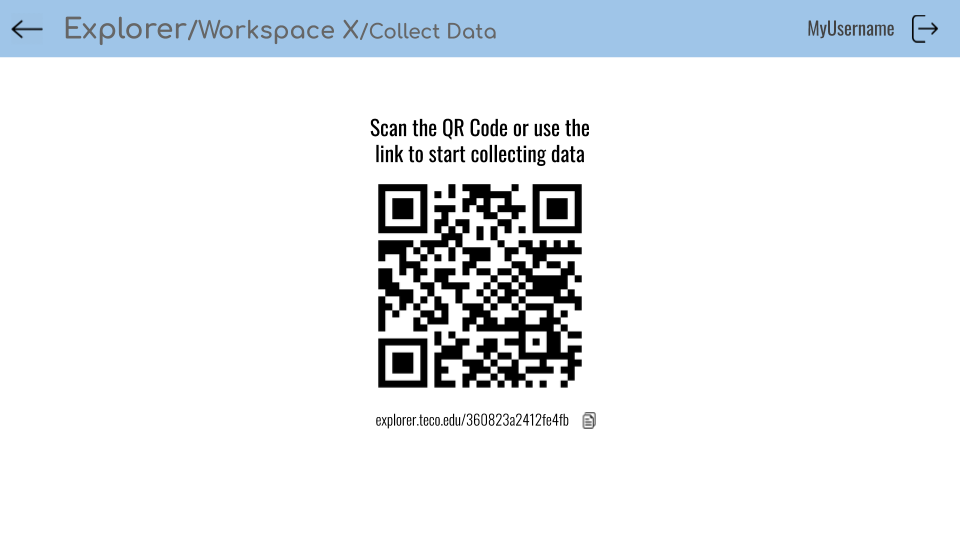
\includegraphics[width = .98\textwidth]{mockups/5.png}}
    \caption{Labels overview}
    \label{fig:labels-overview}
\end{figure}

\begin{figure}[ht]
    \centering
    \fbox{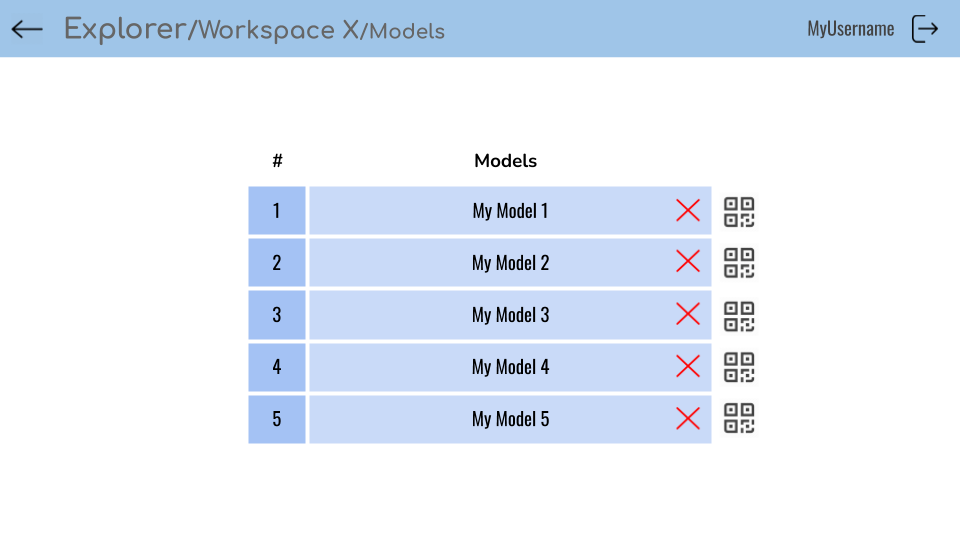
\includegraphics[width = .98\textwidth]{mockups/7.png}}
    \caption{Trained models overview}
    \label{fig:models-overview}
\end{figure}

\begin{figure}[ht]
    \centering
    \fbox{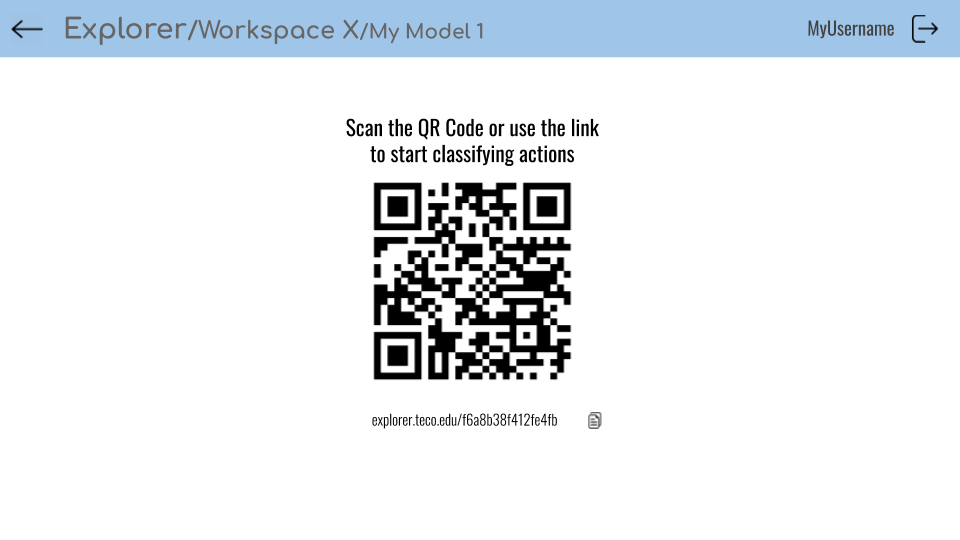
\includegraphics[width = .98\textwidth]{mockups/8.png}}
    \caption{QR Code/Link of trained model to classify data}
    \label{fig:model-link}
\end{figure}

\begin{figure}[ht]
    \centering
    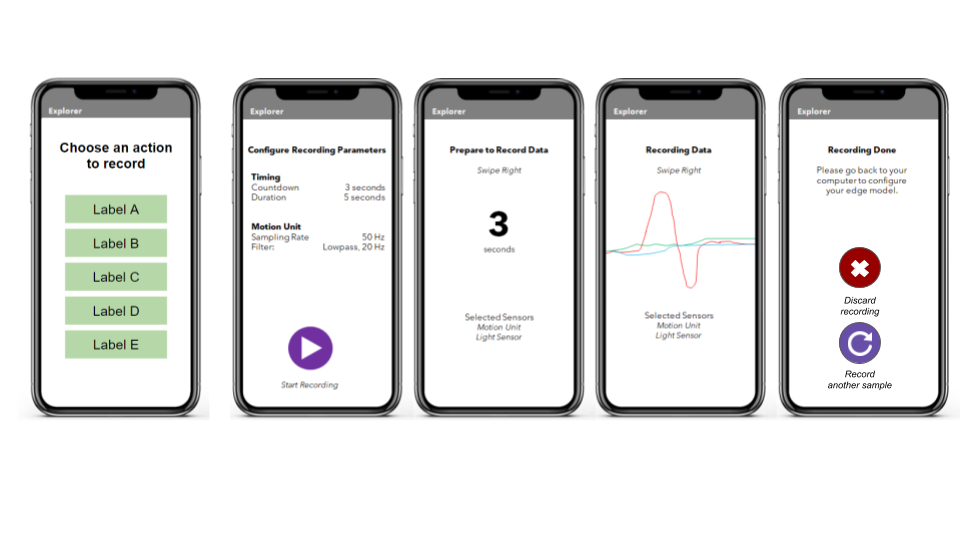
\includegraphics[width = \textwidth]{mockups/9.png}
    \caption{Data collection in mobile}
    \label{fig:mobile}
\end{figure}